\subsection{Three virtual reality T-mazes with varying cognitive demands}
\label{sec:glmhmm:2.2.3}
We next considered the possibility that, rather than contributing directly to a motor output, endogenous activity in DMS pathways may instead have opposing influence over decisions in a manner that is dependent on cognitive demand. To test this idea, we trained mice to perform a set of VR-based, decision-making tasks \cite{pinto_accumulation--evidence_2018} that shared identical motor readouts (left or right choice), had highly similar sensory environments, and yet differed in their cognitive requirements (Fig. \ref{fig:glmhmm:2}a,b).

The first task was an ‘evidence accumulation’ task, in which visuo-tactile cues were transiently presented on each side of the central stem of a virtual T-maze according to a Poisson distribution (‘cue region’, 0–200cm), and mice were rewarded for turning to the maze side with the greater number of cues (Fig. \ref{fig:glmhmm:2}a,b; black). Thus, mice were required to continually accumulate sensory cues over several seconds into a memory (or motor plan) that guided their left/right decision.

In two additional control tasks, we made modifications intended to weaken the cognitive demands of each task. In the first control task (‘no distractors’), cues were presented on the rewarded maze side during the same maze region (0–200cm) according to the same Poisson distribution, but distractor cues on the side of the non-rewarded arm were omitted (Fig. \ref{fig:glmhmm:2}a,b; magenta). The absence of distractors on the non-rewarded side meant that each cue signaled reward with 100\% probability, and thus gradual evidence accumulation was not required. Further ensuring that evidence accumulation was not required, an additional cue at the end of the maze was present only during the cue period (0–200cm) to signal the rewarded side.

\begin{figure}[t!]
  \begin{center}
    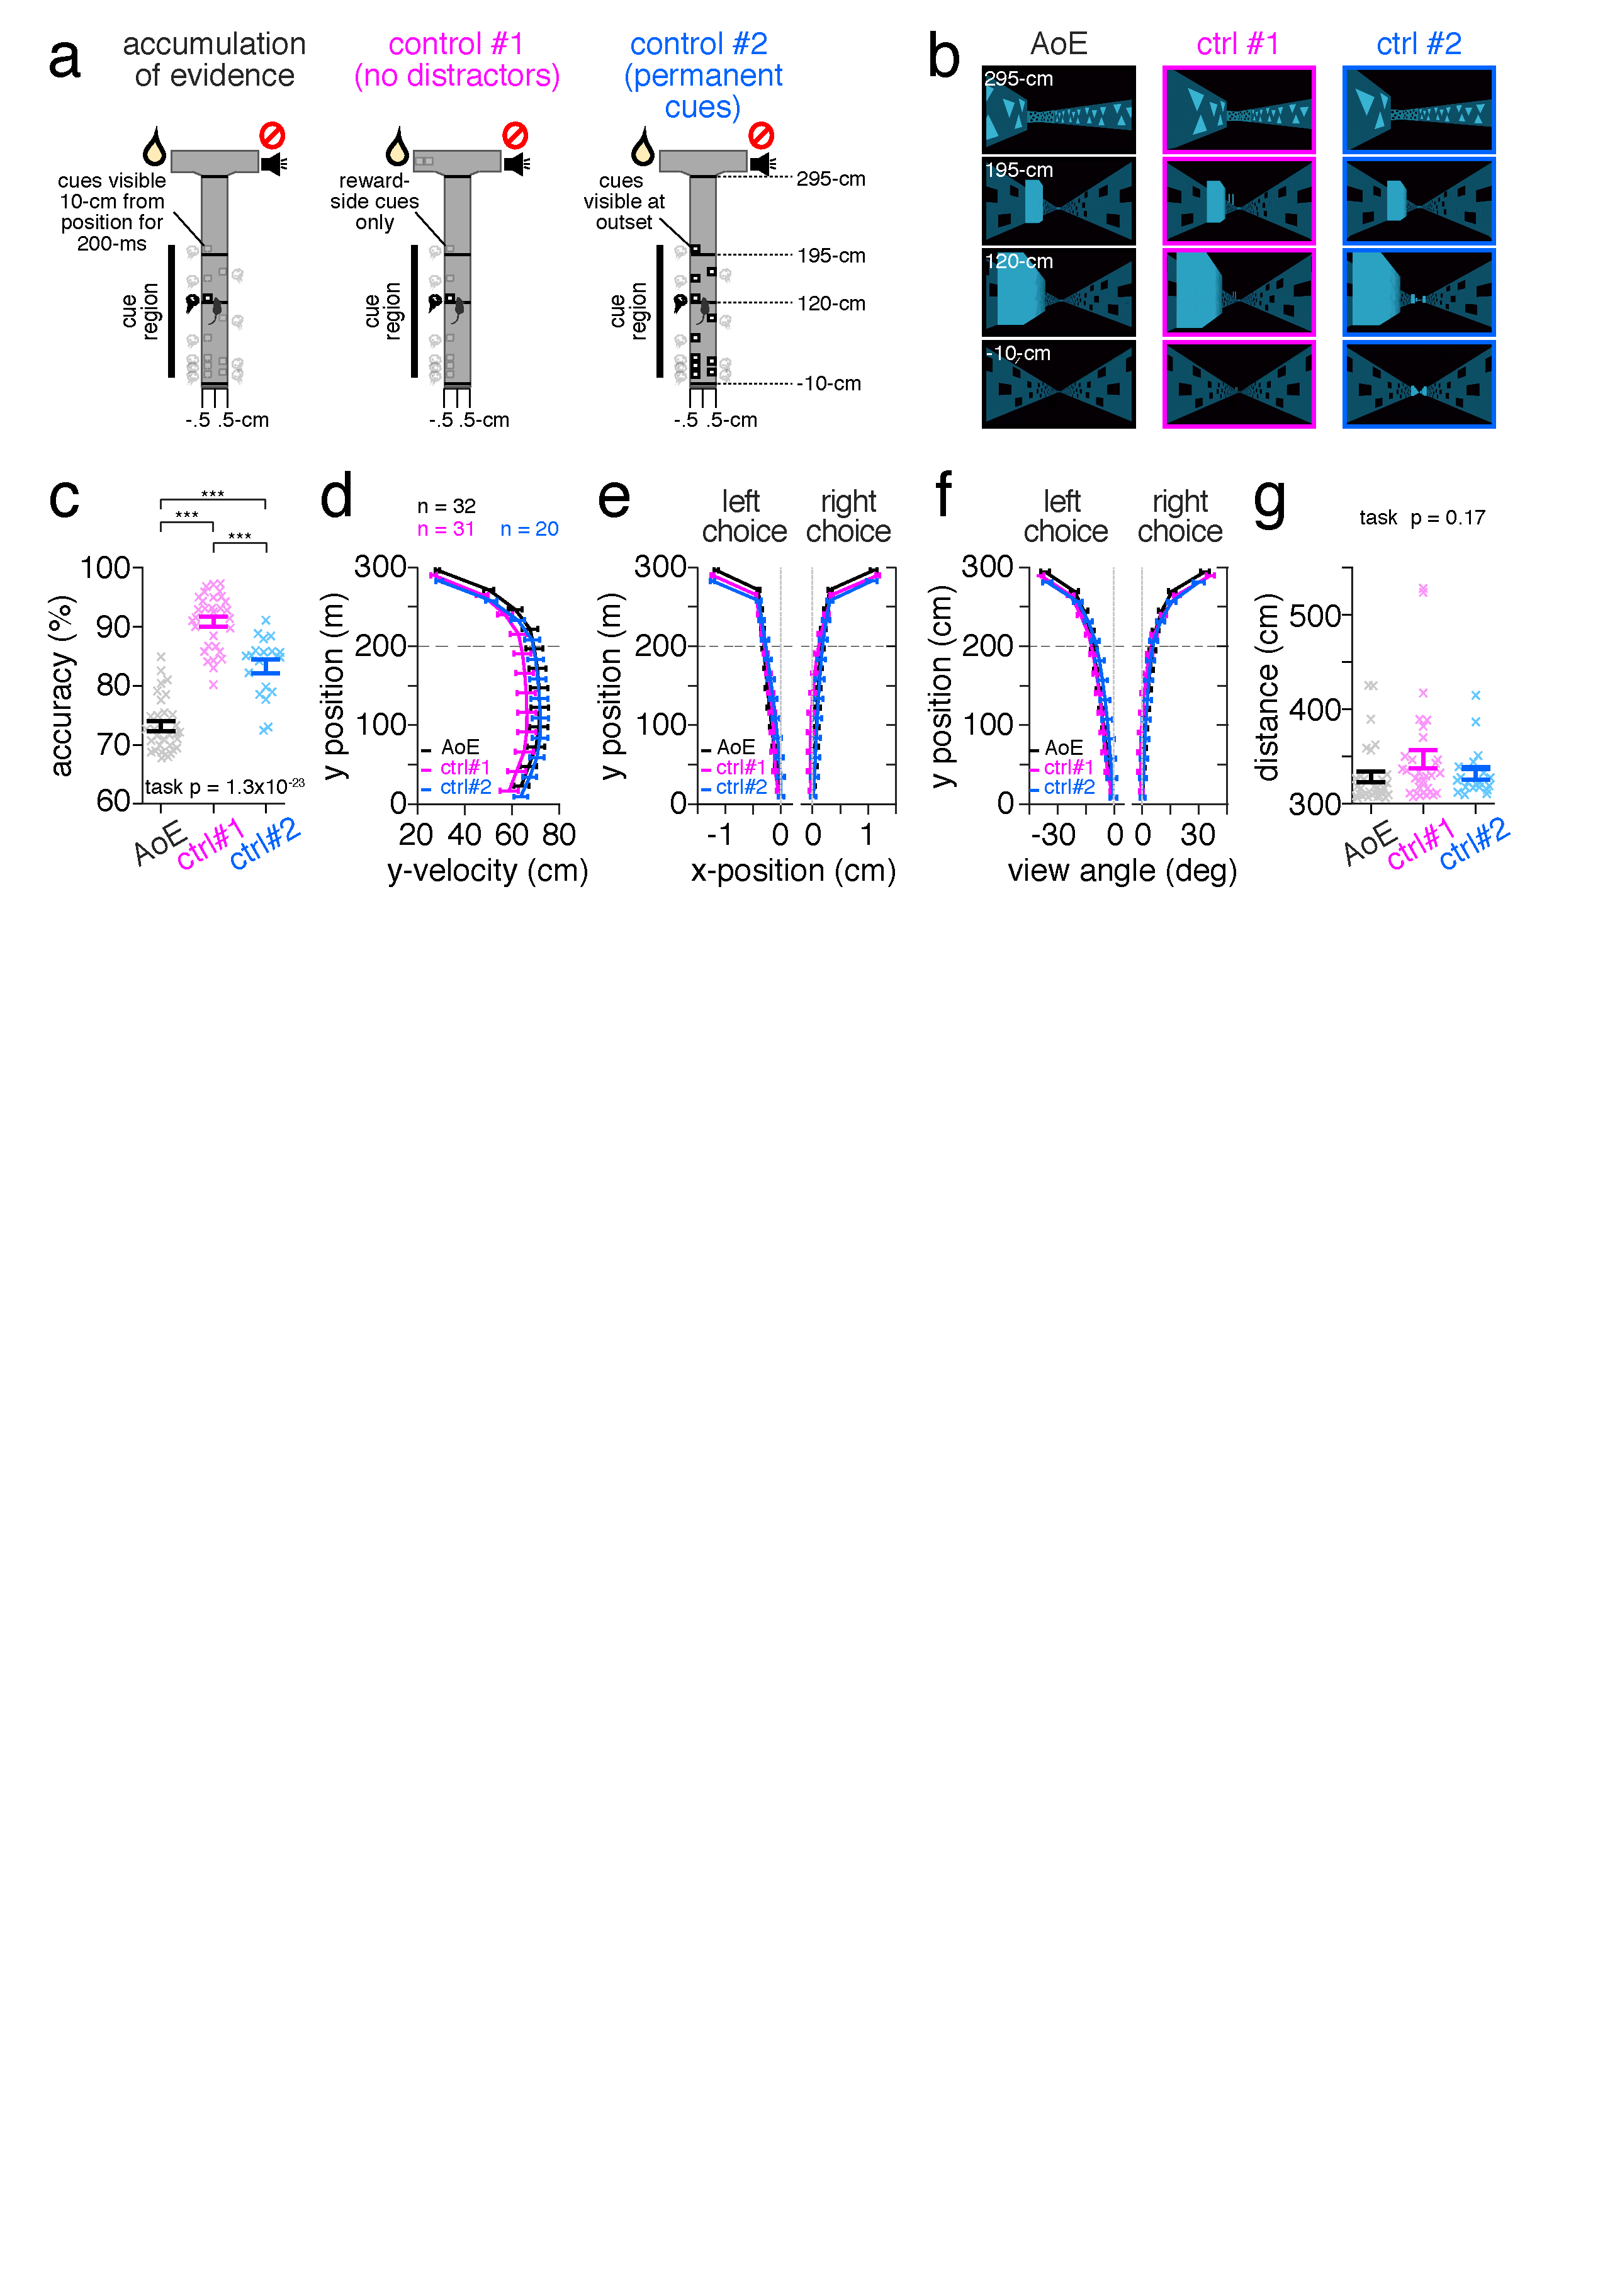
\includegraphics[width=0.90\linewidth]{ch2-glmhmm/glmhmm-figures/Fig2.pdf}
    \caption[A set of virtual reality T-mazes have similar sensory features and identical motor requirements but different cognitive demands]{\textbf{A set of virtual reality T-mazes have similar sensory features and identical motor requirements but different cognitive demands.} (a) Schematic of three virtual reality (VR)-based T-maze tasks. (b) Example mouse perspective  at the same maze position (-10cm, 120cm, 195cm, and 295cm) from the example trial depicted in a of the evidence accumulation (left, black), no distractors (middle, ctrl 1), or permanent cues (right, ctrl 2) tasks. (c) Average choice accuracy (\% correct) across mice performing the accumulation of evidence (black, n = 32 mice, n = 52,381 trials), no distractors (magenta, ctrl 1: n = 31 mice, n = 56,783 trials), or permanent cues (cyan, ctrl 2: n = 20 mice, n = 27,870 trials) tasks. p-value denotes one-way ANOVA of task on accuracy (p = 1.3 x 10-23, F2,80 = 109.4). Asterisks indicate statistical significance of post-hoc, unpaired, two-tailed ranksum comparisons of accuracy between groups (top to bottom: ***p = 3.9 x 10-7, z = -5.1; ***p = 2.1 x 10-11, z = -6.7; ***p = 2.1 x 10-5, z = 4.3). (d) Average y-velocity (cm/s) across mice as a function of y-position (0-300 cm in 25cm bins) during performance of each task (colors and n as in c). (e) Same as d but for average x-position (cm) on left and right choice trials. (f) Same as d but for average view angle (degrees) on left and right choice trials. (g) Average distance (cm) traveled per trial across mice (evidence accumulation, n = 32 mice, n = 53,833 trials; no distractors (control 1): n = 32 mice, n = 60,074 trials; permanent cues (control 2): n = 20 mice, n = 29,192 trials). p-value reflects one-way ANOVA of task on distance (p = 0.16, F2,81 = 1.8). Throughout solid bars denote across mouse mean values $\pm$S.E.M. and transparent ‘x’ indicate individual mouse mean.}
    \label{fig:glmhmm:2}
  \end{center}
  \vspace{-0.5cm}
\end{figure}

In the second control task (‘permanent cues’), the sensory statistics of the cues were identical to those in the evidence accumulation task, but rather than transient visual cue presentation, visual cues were permanently visible from trial onset (Fig. \ref{fig:glmhmm:2}a,b; cyan). This maintained the same conceptual task structure of the evidence accumulation task while decreasing the memory demands, as the sensory cues (or the motor plan) did not need to be remembered until the cues were passed.

We assessed how task demands impacted choice accuracy in each task. Consistent with the greatest cognitive and mnemonic demand in the evidence accumulation task, we found that overall choice accuracy was significantly lower compared to both control tasks (Fig. \ref{fig:glmhmm:2}c, AoE: 73.1 $\pm$ 0.8\%. Ctrl 1: 90.6 $\pm$ 0.9\%. Ctrl 2: 83.3 $\pm$ 1.2\% mean $\pm$ s.e.m).

While the motor requirements of a decision were the same across tasks (crossing an x-position threshold at the end of the central stem; Methods), we examined the possibility that cross-task differences in cognitive requirements altered movement within the stem of the maze (0–300cm). We observed no consistent cross-task differences in velocity, x-position or view angle on left or right choice trials, nor distance traveled (Fig. \ref{fig:glmhmm:2}d–g; see Extended Data Fig. \ref{fig:ap1:ext3}a–f for additional measures). We further compared the relationship between behavior in the stem of the maze and choice across tasks by using a decoder to predict choice based on the trial-by-trial x-position or view angle (Extended Data Fig. \ref{fig:ap1:ext3}g–j) at successive maze positions (0–300cm in 25-cm bins). While we were able to predict choice from either measure above chance levels in all three tasks (consistent with previous studies \cite{pinto_accumulation--evidence_2018}), choice prediction accuracy was statistically indistinguishable across tasks (Extended Data Fig. \ref{fig:ap1:ext3}g–j). Together, this indicated that cross-task differences in task demands did not prompt mice to systematically adopt distinct motor strategies.